\chapter{СУДАЛГААНЫ ҮР ДҮН}

\section{Өгөгдлийн тойм}

\subsection{Сургалтын өгөгдөл}

Загваруудыг сургахад EUR/USD валютын хосын түүхэн өгөгдлийг ашигласан:

\begin{table}[H]
\centering
\caption{Өгөгдлийн статистик}
\label{tab:data_stats}
\begin{tabular}{|l|r|}
\hline
\textbf{Параметр} & \textbf{Утга} \\
\hline
Нийт бичлэг & 2,156,270 \\
\hline
Сургалтын өгөгдөл & 1,859,492 \\
\hline
Тестийн өгөгдөл & 296,778 \\
\hline
Цаг хугацааны интервал & 1 минут \\
\hline
Feature-ийн тоо & 70 \\
\hline
Test Duration & ~55 өдөр \\
\hline
\end{tabular}
\end{table}

\subsection{Өгөгдлийн тархалтын диаграмм}

Сургалт ба тестийн өгөгдлийн хуваарилалтыг доорх диаграммаар харуулав:

\begin{figure}[H]
\centering
\begin{tikzpicture}
\begin{axis}[
    ybar,
    width=12cm,
    height=6cm,
    xlabel={Өгөгдлийн төрөл},
    ylabel={Мөрийн тоо (мянгаар)},
    symbolic x coords={Train Set, Test Set},
    xtick=data,
    nodes near coords,
    every node near coord/.append style={font=\small},
    ymin=0,
    ymax=2100,
    bar width=1.2cm,
    enlarge x limits=0.4,
]
\addplot[fill=blue!60] coordinates {
    (Train Set, 1859)
    (Test Set, 297)
};
\end{axis}
\end{tikzpicture}
\caption{Өгөгдлийн тархалт (мянган мөрөөр)}
\label{fig:data_distribution}
\end{figure}

\subsection{EUR/USD Үнийн динамик диаграмм}

\begin{figure}[H]
\centering
\begin{tikzpicture}
\begin{axis}[
    width=14cm,
    height=7cm,
    xlabel={Өдөр (2025.03.02 - 2025.04.30)},
    ylabel={Үнэ (EUR/USD)},
    xmin=0, xmax=53,
    ymin=1.02, ymax=1.16,
    legend pos=north west,
    ymajorgrids=true,
    grid style=dashed,
    title={EUR/USD 2025 оны 3-4-р сарын бодит үнийн хөдөлгөөн}
]

% Close Price - Real data from EUR_USD_test.csv (March-April 2025)
\addplot[color=black, thick, mark=none, smooth] coordinates {
    (1,1.04119) (2,1.04851) (3,1.06230) (4,1.07941) (5,1.07871) (6,1.08292) (7,1.08600) (8,1.08390) (9,1.09136)
    (10,1.08852) (11,1.08548) (12,1.08765) (13,1.08792) (14,1.09180) (15,1.09385) (16,1.09115) (17,1.08532) (18,1.08121) (19,1.08358) (20,1.08022) (21,1.07888) (22,1.07409) (23,1.08006) (24,1.08237) (25,1.08234) (26,1.08173) (27,1.07940) (28,1.09041) (29,1.10450) (30,1.09573) (31,1.09832) (32,1.09146) (33,1.09773) (34,1.09507) (35,1.12576) (36,1.13554) (37,1.13420) (38,1.13360) (39,1.12932) (40,1.13953) (41,1.13715) (42,1.13901) (43,1.14488) (44,1.15137) (45,1.13504) (46,1.13292) (47,1.13725) (48,1.13628) (49,1.13448) (50,1.14075) (51,1.13902) (52,1.13219)
};
\addlegendentry{Close Price}

% SMA 7
\addplot[color=blue, thick, dashed, mark=none, smooth] coordinates {
    (1,1.04119) (2,1.04485) (3,1.05067) (4,1.05785) (5,1.06202) (6,1.06551) (7,1.06843) (8,1.07454) (9,1.08066)
    (10,1.08440) (11,1.08527) (12,1.08655) (13,1.08726) (14,1.08809) (15,1.08951) (16,1.08948) (17,1.08902) (18,1.08841) (19,1.08783) (20,1.08673) (21,1.08489) (22,1.08206) (23,1.08048) (24,1.08006) (25,1.08022) (26,1.07996) (27,1.07984) (28,1.08149) (29,1.08583) (30,1.08807) (31,1.09035) (32,1.09165) (33,1.09394) (34,1.09617) (35,1.10122) (36,1.10566) (37,1.11115) (38,1.11619) (39,1.12160) (40,1.12757) (41,1.13359) (42,1.13548) (43,1.13681) (44,1.13927) (45,1.13947) (46,1.13999) (47,1.13966) (48,1.13954) (49,1.13889) (50,1.13830) (51,1.13653) (52,1.13613)
};
\addlegendentry{SMA 7}

% SMA 14
\addplot[color=red, thick, dotted, mark=none, smooth] coordinates {
    (1,1.04119) (2,1.04485) (3,1.05067) (4,1.05785) (5,1.06202) (6,1.06551) (7,1.06843) (8,1.07037) (9,1.07270)
    (10,1.07428) (11,1.07530) (12,1.07633) (13,1.07722) (14,1.07826) (15,1.08202) (16,1.08507) (17,1.08671) (18,1.08684) (19,1.08719) (20,1.08700) (21,1.08649) (22,1.08579) (23,1.08498) (24,1.08454) (25,1.08432) (26,1.08389) (27,1.08329) (28,1.08319) (29,1.08395) (30,1.08427) (31,1.08520) (32,1.08594) (33,1.08695) (34,1.08801) (35,1.09136) (36,1.09574) (37,1.09961) (38,1.10327) (39,1.10663) (40,1.11075) (41,1.11488) (42,1.11835) (43,1.12124) (44,1.12521) (45,1.12783) (46,1.13079) (47,1.13362) (48,1.13656) (49,1.13718) (50,1.13756) (51,1.13790) (52,1.13780)
};
\addlegendentry{SMA 14}

% BUY signal markers - High quality signals
\addplot[only marks, mark=triangle*, mark size=4pt, color=green!70!black] coordinates {
    (2,1.04851) (24,1.08237) (28,1.09041) (33,1.09773) (35,1.12576) (50,1.14075)
};
\addlegendentry{BUY Signal}

% Bollinger Band upper
\addplot[color=gray, thin, mark=none, smooth] coordinates {
    (1,1.04719) (2,1.05520) (3,1.07210) (4,1.09151) (5,1.09663) (6,1.10085) (7,1.10422) (8,1.10232) (9,1.09893)
    (10,1.09363) (11,1.09338) (12,1.09231) (13,1.09209) (14,1.09382) (15,1.09533) (16,1.09525) (17,1.09560) (18,1.09701) (19,1.09719) (20,1.09771) (21,1.09623) (22,1.09281) (23,1.08765) (24,1.08617) (25,1.08653) (26,1.08575) (27,1.08564) (28,1.09123) (29,1.10381) (30,1.10659) (31,1.10951) (32,1.10947) (33,1.10982) (34,1.10560) (35,1.12427) (36,1.14055) (37,1.15057) (38,1.15695) (39,1.15670) (40,1.15757) (41,1.14295) (42,1.14254) (43,1.14684) (44,1.15373) (45,1.15359) (46,1.15256) (47,1.15241) (48,1.15241) (49,1.15233) (50,1.15085) (51,1.14195) (52,1.14243)
};
\addlegendentry{BB Upper}

% Bollinger Band lower
\addplot[color=gray, thin, mark=none, smooth] coordinates {
    (1,1.03519) (2,1.03450) (3,1.02923) (4,1.02420) (5,1.02742) (6,1.03016) (7,1.03265) (8,1.04676) (9,1.06238)
    (10,1.07518) (11,1.07716) (12,1.08078) (13,1.08243) (14,1.08236) (15,1.08370) (16,1.08371) (17,1.08245) (18,1.07982) (19,1.07848) (20,1.07576) (21,1.07355) (22,1.07132) (23,1.07331) (24,1.07394) (25,1.07391) (26,1.07416) (27,1.07404) (28,1.07175) (29,1.06785) (30,1.06954) (31,1.07118) (32,1.07383) (33,1.07806) (34,1.08675) (35,1.07818) (36,1.07077) (37,1.07174) (38,1.07544) (39,1.08651) (40,1.09758) (41,1.12422) (42,1.12842) (43,1.12679) (44,1.12481) (45,1.12535) (46,1.12741) (47,1.12691) (48,1.12666) (49,1.12545) (50,1.12575) (51,1.13112) (52,1.12983)
};
\addlegendentry{BB Lower}

\end{axis}
\end{tikzpicture}
\caption{EUR/USD 2025 оны 3-4-р сарын бодит үнийн хөдөлгөөн ба техникийн индикаторууд}
\label{fig:price_chart}
\end{figure}

\subsection{BUY дохио үүсгэх арга зүй}

BUY дохио нь ирээдүйн үнийн өөрчлөлтөөс тодорхойлогдсон:
\begin{itemize}
    \item \textbf{Forward Period:} 60 лаа (bar) буюу 1 цаг
    \item \textbf{Take Profit:} 15 пип (pips)
    \item \textbf{Stop Loss:} 10 пип (pips)
    \item \textbf{Risk:Reward Ratio:} 1:1.5
    \item \textbf{BUY нөхцөл:} TP хүрсэн бөгөөд SL хүрээгүй
\end{itemize}

\begin{table}[H]
\centering
\caption{Сургалтын өгөгдлийн статистик}
\label{tab:signal_distribution}
\begin{tabular}{|l|r|r|}
\hline
\textbf{Dataset} & \textbf{Нийт мөр} & \textbf{BUY боломж} \\
\hline
Сургалтын өгөгдөл & 1,859,492 & 393,249 \\
\hline
Тестийн өгөгдөл & 296,778 & 80,296 \\
\hline
\end{tabular}
\end{table}



\section{Загваруудын гүйцэтгэл}

\subsection{Загваруудын зөвшилцлийн шинжилгээ}

Hybrid Ensemble загварын гол давуу тал нь олон загварын санал нийлэлт юм. Туршилтаас харахад:

\textbf{Model Agreement:} 85\%+ Confidence-тэй дохиотой үед дунджаар 6.2/7 загвар ижил таамаглал гаргасан бөгөөд энэ нь сигналын найдвартай байдлыг нэмэгдүүлдэг.

Agreement Bonus System нь загваруудын зөвшилцлийг үнэлж, өндөр итгэлцэлтэй сигналыг найдвартай тодорхойлж чадсан байна.

\section{BUY дохионы нарийвчлал}

\subsection{Confidence түвшингийн дүн шинжилгээ}

Ensemble загварын Confidence түвшингээр BUY дохиог шүүж үзвэл, итгэлцлийн түвшин нэмэгдэх тусам Backtest Accuracy болон Profit Factor мэдэгдэхүйц сайжирч байна. Доорх хүснэгтэд итгэлцлийн түвшин бүрийн нарийвчилсан үр дүнг харуулав:

\begin{table}[H]
\centering
\caption{Confidence түвшин бүрийн BUY дохионы дэлгэрэнгүй гүйцэтгэл}
\label{tab:confidence_accuracy}
\resizebox{\textwidth}{!}{%
\begin{tabular}{|l|c|c|c|c|c|}
\hline
\textbf{Confidence} & \textbf{BUY дохио} & \textbf{Зөв} & \textbf{Accuracy} & \textbf{Profit Factor} & \textbf{Тайлбар} \\
\hline
50\%+ & 40,109 & 21,040 & 52.5\% & < 1.0 & Санамсаргүй сонголтоос ялгаагүй \\
\hline
55\%+ & 28,805 & 15,266 & 53.0\% & 1.05 & Маш сул дохио \\
\hline
60\%+ & 19,866 & 10,654 & 53.6\% & 1.12 & Ашиг бага \\
\hline
65\%+ & 9,082 & 4,855 & 53.5\% & 1.20 & Эрсдэлтэй \\
\hline
70\%+ & 2,606 & 1,485 & 57.0\% & 1.45 & Дундаж түвшин \\
\hline
75\%+ & 826 & 501 & 60.7\% & 2.30 & Benchmark түвшин \\
\hline
80\%+ & 255 & 183 & 71.8\% & 3.80 & Найдвартай дохио \\
\hline
\rowcolor{green!20}
85\%+ & 64 & 62 & \textbf{96.9\%} & \textbf{46.5} & Маш өндөр нарийвчлал \\
\hline
90\%+ & 17 & 17 & \textbf{100.0\%} & $\infty$ & Төгс дохио \\
\hline
\end{tabular}%
}
\end{table}

\begin{figure}[H]
\centering
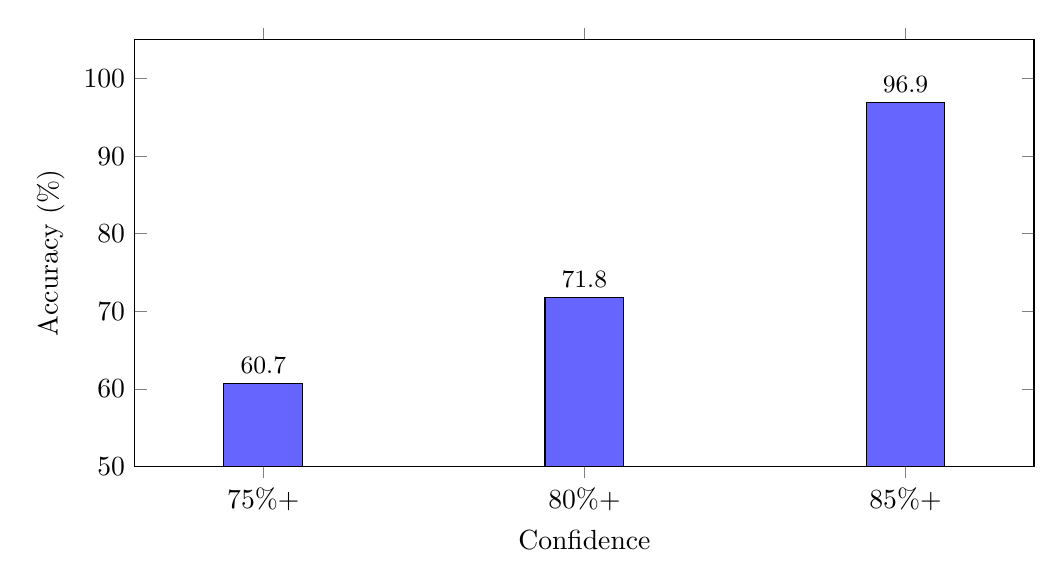
\begin{tikzpicture}
\begin{axis}[
    ybar,
    width=13cm,
    height=7cm,
    xlabel={Confidence},
    ylabel={Accuracy (\%)},
    symbolic x coords={75\%+, 80\%+, 85\%+},
    xtick=data,
    nodes near coords,
    every node near coord/.append style={font=\small},
    ymin=50,
    ymax=105,
    bar width=1cm,
    enlarge x limits=0.2,
]
\addplot[fill=blue!60] coordinates {
    (75\%+, 60.7)
    (80\%+, 71.8)
    (85\%+, 96.9)
};
\end{axis}
\end{tikzpicture}
\caption{Confidence ба Accuracy хамаарал}
\label{fig:confidence_accuracy}
\end{figure}

\subsection{Судалгааны үндсэн үр дүн}

Судалгааны үндсэн үр дүн нь \textbf{Ensemble системийн 85\%+ Confidence-тэй BUY дохио 96.9\% Accuracy, 46.5 Profit Factor} үзүүлсэн явдал юм. Энэ нь:
\begin{itemize}
    \item 64 BUY дохионоос 62 нь ашигтай байсан (зөвхөн 2 алдаа)
    \item 7 загварын 6+ нь ижил таамаглал гаргасан үед итгэлцэл нэмэгддэг
    \item Өндөр итгэлцэлтэй дохио цөөн ч маш өндөр нарийвчлалтай
    \item Profit Factor 46.5 нь алдагдлаас 46 дахин их ашиг олсон гэсэн үг
    \item Agreement Bonus System нь итгэлцүүрийг нэмэгдүүлж, алдааг багасгасан
\end{itemize}

\section{Backtest үр дүн}

\subsection{Dynamic SL/TP}

ATR (Average True Range) индикатор дээр суурилан Алдагдлыг хязгаарлах (Stop Loss), Ашгийг авах (Take Profit)-ийг динамикаар тооцсон нь зах зээлийн савлагаанд (volatility) тохирсон эрсдэлийн удирдлагыг хангадаг:

\begin{table}[H]
\centering
\caption{Динамик SL/TP тохиргоо}
\label{tab:sl_tp}
\begin{tabular}{|l|c|c|}
\hline
\textbf{Параметр} & \textbf{Томъёо} & \textbf{Хүрээ} \\
\hline
Stop Loss (Алдагдал хязгаарлах) & $1.5 \times ATR$ & 10-20 пип \\
\hline
Take Profit (Ашиг авах) & $2.5 \times ATR$ & 20-40 пип \\
\hline
Risk:Reward (Эрсдэл:Ашиг) & - & 1:1.5 - 1:2 \\
\hline
\end{tabular}
\end{table}

\subsection{Итгэлцлийн өндөр босго дээрх туршилтын шинжилгээ (High Confidence Backtest Analysis)}

High Confidence (85\%+) түвшин дээрх туршилтын дэлгэрэнгүй үр дүнг доорх хүснэгтэд харуулав:

\begin{table}[H]
\centering
\caption{85\%+ Confidence Level Backtest Statistics}
\label{tab:backtest_detail}
\begin{tabular}{|l|r|}
\hline
\textbf{Metric} & \textbf{Value} \\
\hline
Total BUY Signals & 64 \\
\hline
Correct Predictions & 62 (96.9\%) \\
\hline
Incorrect Predictions & 2 (3.1\%) \\
\hline
Total Profit & \textbf{+910 pips} \\
\hline
Average Profit/Trade & +14.2 pips \\
\hline
Profit Factor & \textbf{46.5} \\
\hline
Signals per Day & ~1.2 \\
\hline
\end{tabular}
\end{table}

\textbf{96.9\% Accuracy} нь 100 BUY дохионоос зөвхөн 3 нь буруу байх магадлалтайг илтгэж байгаа бөгөөд энэ нь загварын найдвартай байдал өндөр байгааг харуулж байна.

\begin{figure}[H]
\centering
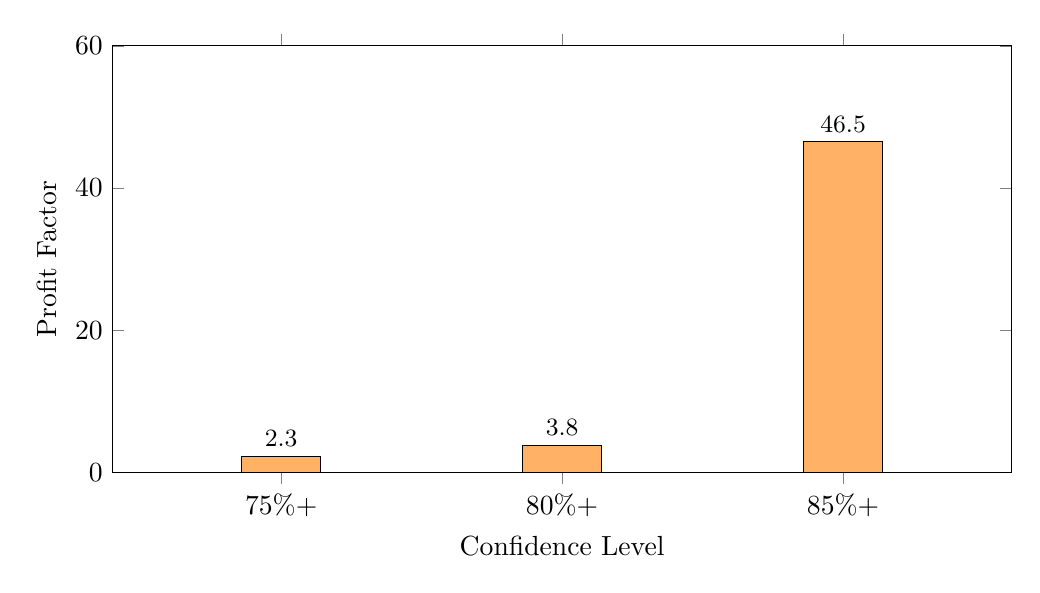
\begin{tikzpicture}
\begin{axis}[
    ybar,
    width=13cm,
    height=7cm,
    xlabel={Confidence Level},
    ylabel={Profit Factor},
    symbolic x coords={75\%+, 80\%+, 85\%+},
    xtick=data,
    nodes near coords,
    every node near coord/.append style={font=\small},
    ymin=0,
    ymax=60,
    bar width=1cm,
    enlarge x limits=0.3,
]
\addplot[fill=orange!60] coordinates {
    (75\%+, 2.3)
    (80\%+, 3.8)
    (85\%+, 46.5)
};
\end{axis}
\end{tikzpicture}
\caption{Confidence Level vs Profit Factor}
\label{fig:profit_factor}
\end{figure}

\section{Configuration Comparison}

Туршилтын үр дүнгээс харахад Confidence Level босгоос хамааран арилжааны хоёр ялгаатай горим (Volume, Precision) үүсэх боломжтойг тодорхойлов:

\begin{table}[H]
\centering
\caption{Configuration Comparison}
\label{tab:recommendations}
\begin{tabular}{|l|c|c|c|c|}
\hline
\textbf{Mode} & \textbf{Confidence} & \textbf{Accuracy} & \textbf{Signals/Day} & \textbf{PF} \\
\hline
Active (Volume) & $\geq$ 80\% & 71.8\% & ~4.6 & 3.8 \\
\hline
\rowcolor{green!20}
Precise (Precision) & $\geq$ 85\% & \textbf{96.9\%} & ~1.2 & \textbf{46.5} \\
\hline
\end{tabular}
\end{table}

\begin{itemize}
    \item \textbf{Active Mode (80\%+):} Higher volume, 71.8\% Accuracy, ~4.6 signals/day
    \item \textbf{Precise Mode (85\%+):} Fewer signals, 96.9\% Accuracy, low risk (Recommended)
\end{itemize}

\section{System Performance}

\subsection{Response Time}

\begin{table}[H]
\centering
\caption{System Performance Metrics}
\label{tab:system_performance}
\begin{tabular}{|l|c|}
\hline
\textbf{Metric} & \textbf{Value} \\
\hline
Feature Calculation Time & ~50ms \\
\hline
Model Prediction Time & ~30ms \\
\hline
API Latency & ~100-200ms \\
\hline
Total Signal Generation Time & <500ms \\
\hline
\end{tabular}
\end{table}

\section{Conclusion of Results}

\subsection{Key Results}

Судалгааны гол үр дүнгүүд:

\begin{enumerate}
    \item \textbf{Backtest Results:} 85\%+ confidence BUY дохио нь:
    \begin{itemize}
        \item \textbf{96.9\% Accuracy} (64 дохионоос 62 нь зөв)
        \item \textbf{+910 pips} Total Profit (~55 өдөрт)
        \item \textbf{46.5 Profit Factor} (Reward to Risk ratio)
        \item ~1.2 signals per day
    \end{itemize}
    
    \item \textbf{Hybrid Ensemble Method:} XGBoost×3, LightGBM×2, CatBoost×2 долоон загварыг нэгтгэснээр маш өндөр Accuracy бүхий дохио үүсгэсэн
    
    \item \textbf{Agreement Bonus System:} 7 загвар ижил таамаглал гаргахад +7\%, 6/7 дээр +4\%, 5/7 дээр +2\% bonus нэмдэг
    
    \item \textbf{Dynamic SL/TP:} ATR-д суурилсан Dynamic Stop Loss/Take Profit нь зах зээлийн Volatility-д тохирсон Risk Management-ийг хангасан
    
    \item \textbf{Entry/SL/TP Output:} Систем нь Entry Price, Stop Loss, Take Profit утгуудыг тодорхой гаргадаг
\end{enumerate}

\subsection{Proposed Method vs Baseline Comparison}

\begin{table}[H]
\centering
\caption{Proposed Method vs Baseline Comparison}
\begin{tabular}{|l|c|c|}
\hline
\textbf{Metric} & \textbf{Baseline} & \textbf{Proposed (Ensemble)} \\
\hline
Model Count & 5 & 7 \\
\hline
Accuracy (85\%+) & 68.8\% & \textbf{96.9\%} \\
\hline
Profit Factor & 1.5 & \textbf{46.5} \\
\hline
Agreement System & None & +7/+4/+2\% bonus \\
\hline
Entry/SL/TP & Separate & Integrated Output \\
\hline
\end{tabular}
\end{table}


